%%%%%%%%%%%%%%%%%%%%%%%%%%%%%%%%%%%%%%%%%%%%%%%%%%%%%%%%%%%%%%%
%
% Welcome to Overleaf --- just edit your LaTeX on the left,
% and we'll compile it for you on the right. If you give
% someone the link to this page, they can edit at the same
% time. See the help menu above for more info. Enjoy!
%
% Note: you can export the pdf to see the result at full
% resolution.
%
%%%%%%%%%%%%%%%%%%%%%%%%%%%%%%%%%%%%%%%%%%%%%%%%%%%%%%%%%%%%%%%
% Author: Till Tantau
% Source: The PGF/TikZ manual

\documentclass{article}

\usepackage{pgf}
\usepackage{tikz}
\usetikzlibrary{arrows,automata}
\usepackage[latin1]{inputenc}
\usepackage{verbatim}
\usepackage{tkz-berge}
\usetikzlibrary{graphs,graphs.standard}



\begin{document}



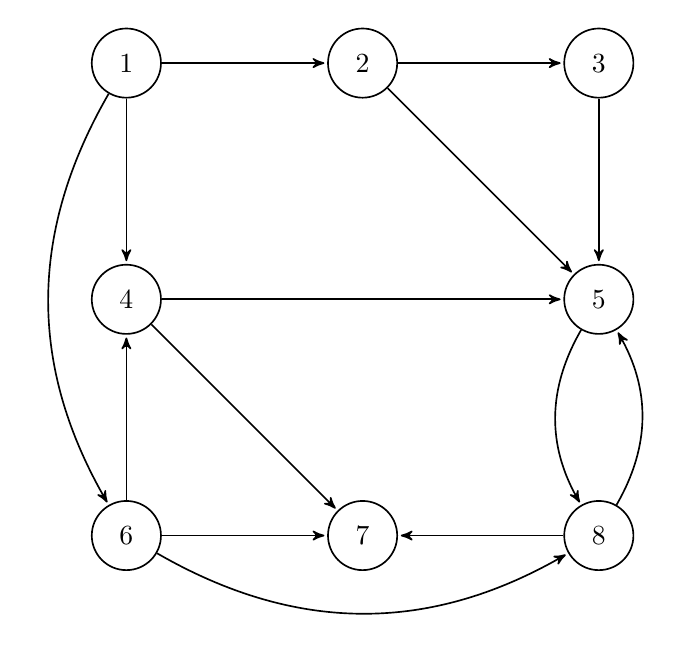
\begin{tikzpicture}[->,>=stealth',shorten >=1pt,auto,node distance=3cm,
                    semithick]
\tikzstyle{every state}=[fill=white,draw=black,text=black]
\node[state] (1) {$1$};
\node[state] (2) [right of=1] {$2$};
\node[state] (3) [right of=2] {$3$};
\node[state] (4) [below of=1] {$4$};
\node[state] (5) [below of=3] {$5$};
\node[state] (6) [below of=4] {$6$};
\node[state] (7) [right of=6] {$7$};
\node[state] (8) [right of=7] {$8$};
\path (1) edge node{} (2)
          edge node{} (4)
          edge [bend right] node{} (6)
      (2) edge node{} (3)
          edge node{} (5)
      (3) edge node{} (5)
      (4) edge node{} (7)
          edge node{} (5)
      (5) edge [bend right] node{} (8)
      (6) edge node{} (4)
          edge node{} (7)
          edge [bend right] node{} (8)
      (8) edge [bend right] node{} (5)
          edge node{} (7);
          
\end{tikzpicture}


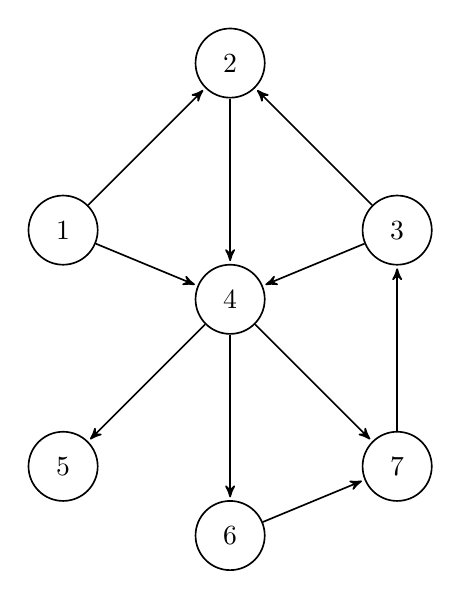
\begin{tikzpicture}[->,>=stealth',shorten >=1pt,auto,node distance=3cm,
semithick]
\tikzstyle{every state}=[fill=white,draw=black,text=black]
\node[state] (1) {$1$};
\node[state] (2) [above right of=1] {$2$};
\node[state] (3) [below right of=2] {$3$};
\node[state] (4) [below of=2] {$4$};
\node[state] (5) [below left of=4] {$5$};
\node[state] (6) [below of=4] {$6$};
\node[state] (7) [below right of=4] {$7$};
\path (1) edge node{} (2)
          edge node{} (4)
      (2) edge node{} (4)
      (3) edge node{} (2)
          edge node{} (4)
      (4) edge node{} (5)
          edge node{} (6)
          edge node{} (7)
      (6) edge node{} (7)
      (7) edge node{} (3);

\end{tikzpicture}


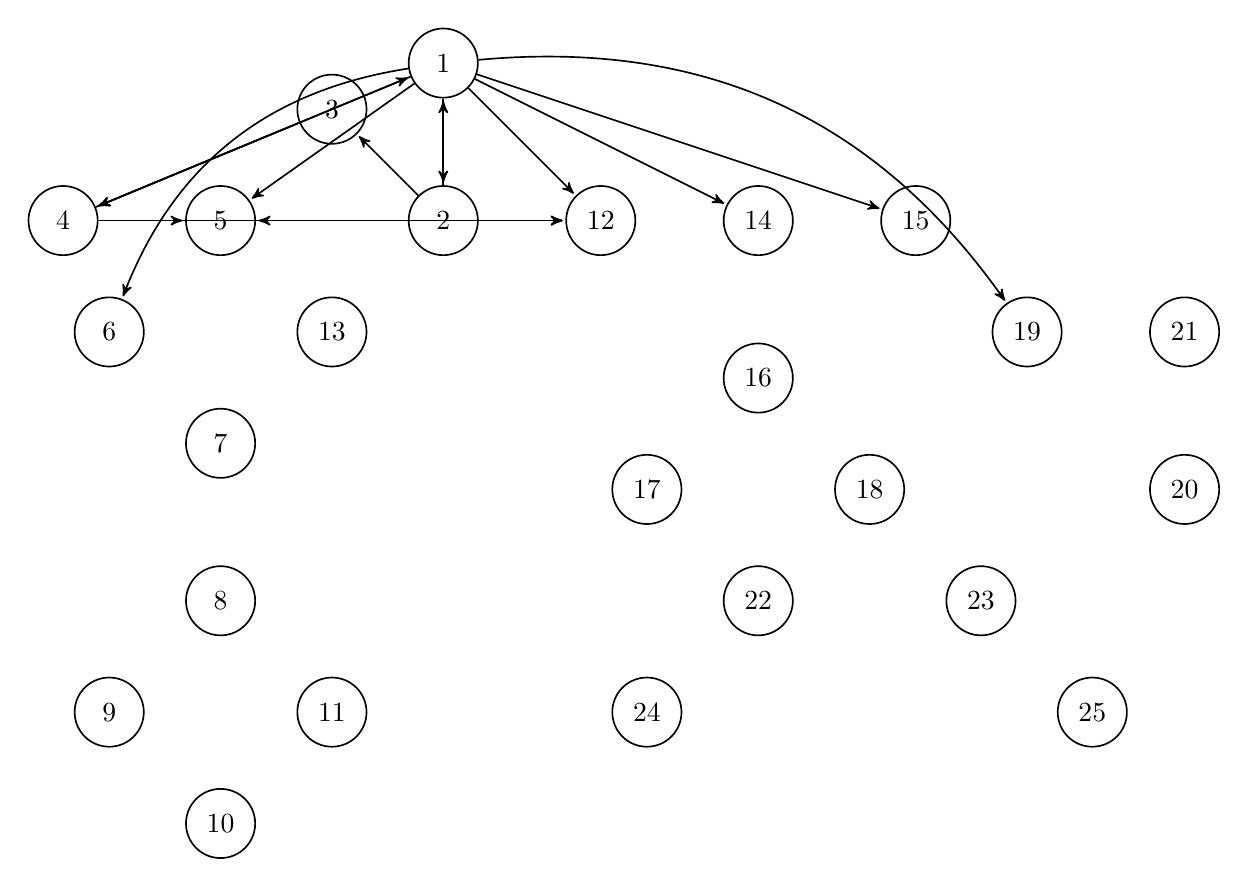
\begin{tikzpicture}[->,>=stealth',shorten >=1pt,auto,node distance = 2cm,
semithick]
\tikzstyle{every state}=[fill=white,draw=black,text=black]
\node[state] (1)  {$1$};
\node[state] (2)  [below of=1] {$2$};
\node[state] (3)  [above left of=2] {$3$};
\node[state] (5)  [below left of=3] {$5$};
\node[state] (4)  [left of=5] {$4$};
\node[state] (6)  [below left of=5]{$6$};
\node[state] (7)  [below right of=6]{$7$};
\node[state] (8)  [below of=7]{$8$};
\node[state] (9)  [below left of=8]{$9$};
\node[state] (10) [below right of=9]{$10$};
\node[state] (11) [below right of=8]{$11$};
\node[state] (12) [right of=2]{$12$};
\node[state] (13) [below right of=5]{$13$};
\node[state] (14) [right of=12]{$14$};
\node[state] (15) [right of=14]{$15$};
\node[state] (16) [below of=14]{$16$};
\node[state] (17) [below left of=16]{$17$};
\node[state] (18) [below right of=16]{$18$};
\node[state] (19) [below right of=15]{$19$};
\node[state] (21) [right of=19]{$21$};
\node[state] (20) [below of=21]{$20$};
\node[state] (22) [below left of=18]{$22$};
\node[state] (23) [below right of=18]{$23$};
\node[state] (24) [below left of=22]{$24$};
\node[state] (25) [below right of=23]{$25$};
\path (1) edge [bend right] node{} (6)
          edge node{} (4)
          edge node{} (5)
          edge node{} (2)
          edge node{} (12)
          edge node{} (14)
          edge node{} (15)
          edge [bend left] node{}  (19)
      (2) edge node{} (1)
          edge node{} (12)
          edge node{} (3)
          edge node{} (5)
      (3) edge node{} (4)
      (4) edge node{} (1)
          edge node{} (5)
          edge node{} (12)
     ;
  \end{tikzpicture}
  
\newpage
 \begin{tikzpicture}
   \tikz \graph [grow down, branch right sep] {
1 -> { 6 ->{1,7,8}
4,5,2,12,14,15,19} -> 25
};
  \end{tikzpicture}


\newpage
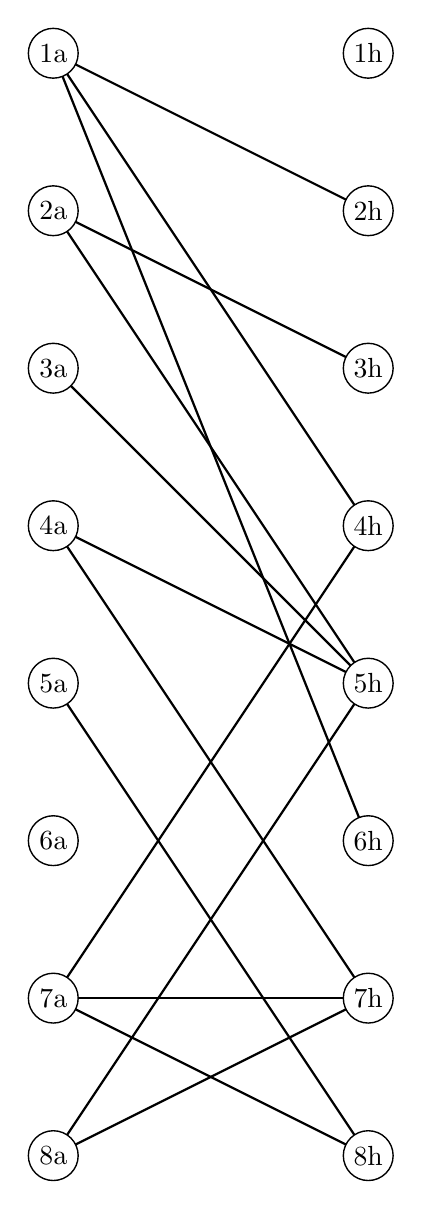
\begin{tikzpicture}
   \begin{scope}[rotate=90]
       \SetVertexNoLabel
       \grEmptyLadder[RA=2,RB=4]{8}   
       \AssignVertexLabel{a}{8h,7h,6h,5h,4h,3h,2h,1h}
       \AssignVertexLabel{b}{8a,7a,6a,5a,4a,3a,2a,1a}

   \end{scope} 
   \EdgeFromOneToSel{b}{a}{0}{1,3}
   \EdgeFromOneToSel{b}{a}{1}{0,1,4}
   \EdgeFromOneToSel{b}{a}{3}{0}
   \EdgeFromOneToSel{b}{a}{4}{1,3} 
   \EdgeFromOneToSel{b}{a}{5}{3}
   \EdgeFromOneToSel{b}{a}{6}{5,3}
   \EdgeFromOneToSel{b}{a}{7}{2,4,6} 
\end{tikzpicture} 

\end{document}